% (find-LATEX "2020-1-C2-somas-1.tex")
% (defun c () (interactive) (find-LATEXsh "lualatex -record 2020-1-C2-somas-1.tex" :end))
% (defun D () (interactive) (find-pdf-page      "~/LATEX/2020-1-C2-somas-1.pdf"))
% (defun d () (interactive) (find-pdftools-page "~/LATEX/2020-1-C2-somas-1.pdf"))
% (defun e () (interactive) (find-LATEX "2020-1-C2-somas-1.tex"))
% (defun u () (interactive) (find-latex-upload-links "2020-1-C2-somas-1"))
% (defun v () (interactive) (find-2a '(e) '(d)) (g))
% (find-pdf-page   "~/LATEX/2020-1-C2-somas-1.pdf")
% (find-sh0 "cp -v  ~/LATEX/2020-1-C2-somas-1.pdf /tmp/")
% (find-sh0 "cp -v  ~/LATEX/2020-1-C2-somas-1.pdf /tmp/pen/")
%   file:///home/edrx/LATEX/2020-1-C2-somas-1.pdf
%               file:///tmp/2020-1-C2-somas-1.pdf
%           file:///tmp/pen/2020-1-C2-somas-1.pdf
% http://angg.twu.net/LATEX/2020-1-C2-somas-1.pdf
% (find-LATEX "2019.mk")

% «.defs»		(to "defs")
% «.title»		(to "title")
% «.exercicio-6»	(to "exercicio-6")

\documentclass[oneside,12pt]{article}
\usepackage[colorlinks,citecolor=DarkRed,urlcolor=DarkRed]{hyperref} % (find-es "tex" "hyperref")
\usepackage{amsmath}
\usepackage{amsfonts}
\usepackage{amssymb}
\usepackage{pict2e}
\usepackage[x11names,svgnames]{xcolor} % (find-es "tex" "xcolor")
%\usepackage{colorweb}                 % (find-es "tex" "colorweb")
%\usepackage{tikz}
%
% (find-dn6 "preamble6.lua" "preamble0")
%\usepackage{proof}   % For derivation trees ("%:" lines)
%\input diagxy        % For 2D diagrams ("%D" lines)
%\xyoption{curve}     % For the ".curve=" feature in 2D diagrams
%
\usepackage{edrx15}               % (find-LATEX "edrx15.sty")
\input edrxaccents.tex            % (find-LATEX "edrxaccents.tex")
\input edrxchars.tex              % (find-LATEX "edrxchars.tex")
\input edrxheadfoot.tex           % (find-LATEX "edrxheadfoot.tex")
\input edrxgac2.tex               % (find-LATEX "edrxgac2.tex")
%
%\usepackage[backend=biber,
%   style=alphabetic]{biblatex}            % (find-es "tex" "biber")
%\addbibresource{catsem-slides.bib}        % (find-LATEX "catsem-slides.bib")
%
% (find-es "tex" "geometry")
\usepackage[a6paper, landscape,
            top=1.5cm, bottom=.25cm, left=1cm, right=1cm, includefoot
           ]{geometry}
%
\begin{document}

%\catcode`\^^J=10
%\directlua{dofile "dednat6load.lua"}  % (find-LATEX "dednat6load.lua")

% «defs»  (to ".defs")
% (find-LATEX "edrx15.sty" "colors-2019")
\long\def\ColorRed   #1{{\color{Red1}#1}}
\long\def\ColorViolet#1{{\color{MagentaVioletLight}#1}}
\long\def\ColorViolet#1{{\color{Violet!50!black}#1}}
\long\def\ColorGreen #1{{\color{SpringDarkHard}#1}}
\long\def\ColorGreen #1{{\color{SpringGreenDark}#1}}
\long\def\ColorGreen #1{{\color{SpringGreen4}#1}}
\long\def\ColorGray  #1{{\color{GrayLight}#1}}
\long\def\ColorGray  #1{{\color{black!30!white}#1}}
\long\def\ColorBrown #1{{\color{Brown}#1}}
\long\def\ColorBrown #1{{\color{brown}#1}}

\long\def\ColorShort #1{{\color{SpringGreen4}#1}}
\long\def\ColorLong  #1{{\color{Red1}#1}}

\def\frown{\ensuremath{{=}{(}}}
\def\True {\mathbf{V}}
\def\False{\mathbf{F}}
\def\D    {\displaystyle}

\def\drafturl{http://angg.twu.net/LATEX/2020-1-C2.pdf}
\def\drafturl{http://angg.twu.net/2020.1-C2.html}
\def\draftfooter{\tiny \href{\drafturl}{\jobname{}} \ColorBrown{\shorttoday{} \hours}}

% (find-angg ".emacs" "c2q192")


%  _____ _ _   _                               
% |_   _(_) |_| | ___   _ __   __ _  __ _  ___ 
%   | | | | __| |/ _ \ | '_ \ / _` |/ _` |/ _ \
%   | | | | |_| |  __/ | |_) | (_| | (_| |  __/
%   |_| |_|\__|_|\___| | .__/ \__,_|\__, |\___|
%                      |_|          |___/      
%
% «title»  (to ".title")

\thispagestyle{empty}

\begin{center}

\vspace*{1.2cm}

{\bf \Large Cálculo 2 - 2020.1}

\bsk

Aula 2: Integrais como somas de retângulos (1)

\bsk

Eduardo Ochs - RCN/PURO/UFF

\url{http://angg.twu.net/2020.1-C2.html}

\end{center}

\newpage

{\bf Pra que a gente vai usar integrais e EDOs?}

Pra ser bem honesto:

1. Pra passar em Cálculo 2

2. Em umas poucas matérias depois

3. Em quase nada depois que a gente crescer

\msk

MAAAAAS pra aprender a integrar e resolver EDOs nós vamos precisar
aprender várias coisas que a gente vai usar zilhões de vezes depois do
curso... e o que a gente vai ver hoje, que é {\sl como interpretar
  certos somatórios como áreas e como visualizar essas áreas}, vai ser
incrivelmente útil depois.



\newpage

{\bf Algumas figuras}

Dê uma olhada nas notas de aula da Cristiane Hernández, linkadas na
página do curso... por exemplo,

% (find-c2crishernandezpage (+ 10  2) "")
% (find-latexgimp-links "2020-1-C2/area-hernandez-1")

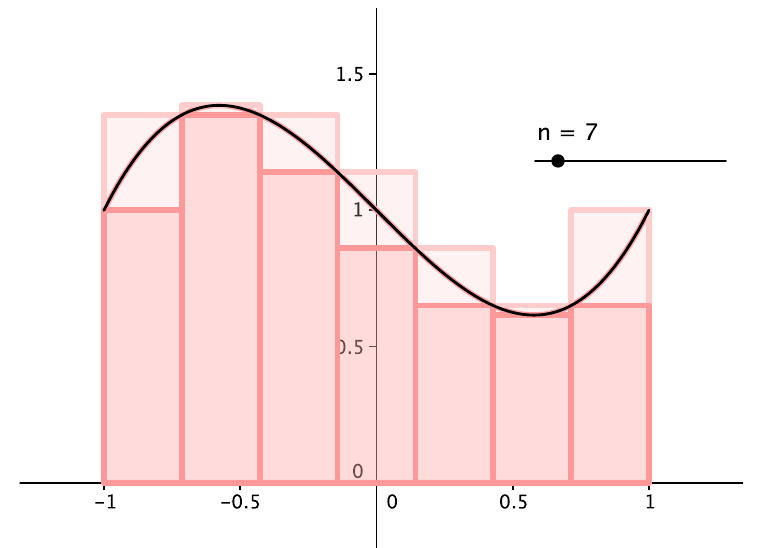
\includegraphics[width=8cm]{2020-1-C2/area-hernandez-1.png}


\newpage

{\bf Nossa função preferida}

Seja $f(x) = 4 - (x-2)^2$.

Isto é uma parábola com a concavidade pra baixo.

Verifique que:

$f(0)=4-4=0$,

$f(1)=4-1=3$,

$f(2)=4-0=4$,

$f(3)=4-1=3$,

$f(4)=4-4=0$.

\msk

Além disso $f'(x) = -2(x-2)$, $f'(1)=2$, $f'(3)=-2$, e

a reta tangente à curva $y=f(x)$ em $x=1$ tem coef.\ angular 2, e

a reta tangente à curva $y=f(x)$ em $x=3$ tem coef.\ angular -2.

\msk

{\bf Exercício 1:} use estas informações para traçar o gráfico de $f(x)$

entre $x=0$ e $x=4$.


\newpage

{\bf Dois jeitos de visualizar $(x,f(x))$}

Jeito burro:

Em $x=2.5$ temos

$f(2.5) = 4 - (2.5-2)^2 = 4 - 0.5^2 = 4-0.25 = 3.75$.

Encontre o ponto $y=3.75$ no eixo $y$.

Desenhe o ponto $(2.5,3.75)$.

\msk

Jeito esperto/rápido:

Encontre no eixo $x$ o ponto $x=2.5$.

Suba esse ponto pra curva $y=f(x)$ --

você encontrou o ponto $(2.5,f(2.5))$!


\newpage

{\bf Mais exercícios}

{\bf Exercício 2.} Desenhe o gráfico da nossa função preferida

(obs: sempre no intervalo entre $x=0$ e $x=4$!)

e desenhe sobre ele o retângulo ``cuja área é $f(0.5)·(1.5-0.5)$''.

Truque: isto é altura $·$ base, e a base vai de $x=0.5$ a $x=1.5$.

\msk

{\bf Exercício 3.} Desenhe em outro gráfico

a nossa função preferida e sobre ela os retângulos da soma abaixo:

$f(0.5)·(1.5-0.5) + f(1.5)·(2-1.5) + f(2)·(3-2) + f(3.5)(3.5-3)$

\newpage

{\bf Partições}

\ColorRed{Informalmente} uma partição de um intervalo $[a,b]$ é um
modo de decompor $[a,b]$ em intervalos menores consecutivos. Por
exemplo, 
%
$$[2,7] = [2,3.5]∪[3.5,4]∪[4,6]∪[6,7]$$

A definição ``certa'' é mais complicada... vamos vê-la daqui a pouco.

Caso geral:
%
$$[a,b] = [a_1,b_1]∪[a_2,b_2]∪\ldots∪[a_N,b_N],$$

onde:

$N$ é o número de intervalos,

$a=a_1$, $b=b_N$, (``extremidades'')

$a_i<b_i$ para todo $i$ em que isto faz sentido ($i=1,\ldots,N$)

$b_i=a_{i+1}$ para todo $i$ e.q.i.f.s.; neste caso, $i=1,\ldots,N-1$

\newpage

{\bf Partições (2)}

Um jeito prático de definir uma partição é usando uma tabela.

Por exemplo, esta tabela
%
$$\begin{array}{ccc}
  i & a_i & b_i \\\hline
  1 & 2 & 3.5 \\
  2 & 3.5 & 4 \\
  3 & 4 & 6 \\
  4 & 6 & 7 \\
  \end{array}
$$

corresponde à partição de $[2,7]$ do slide anterior.

{\bf Exercício 4.} Converta esta ``partição''
%
$$[4,12] = [4,5]∪[5,6]∪[6,9]∪[9,10]∪[10,12]$$

numa tabela. Neste caso quem são $a$, $b$ e $N$?

\newpage

{\bf Partições (3)}

A definição \ColorRed{certa} de partição é a seguinte.

Digamos que $P$ seja um subconjunto não-vazio e finito de $\R$,

e que o menor elemento de $P$ seja $a$ e o maior seja $b$.

Então $P$ é uma \ColorRed{partição} do intervalo $[a,b]$.

\msk

Exemplo: a partição $P=\{2,3.5,4,6,7\}$ corresponde a:
%
$$[2,7] = [2,3.5]∪[3.5,4]∪[4,6]∪[6,7]$$

Pra fazer a tradução ponha os elementos de $P$ em ordem e chame-os de
$b_0,\ldots,b_N$; defina cada $a_i$ como sendo $b_{i-1}$ -- por
exemplo, $a_1 = b_0$ -- e encontre $a$, $b$, e $N$.

\msk

{\bf Exercício 5.} Converta a partição $P=\{2.5,3,4,6,10\}$ para o
formato tabela e para o formato $[a,b] = [a_1,b_1]∪\ldots∪[a_N,b_N].$


\newpage

{\bf Partições definem muitas coisas implicitamente}

Quando dizemos algo como ``Seja $P$ a partição $\{2.5,4,6\}$'' estamos
criando um contexto no qual há uma partição ``default'' definida... e
neste contexto vamos ter valores definidos para $N$, $a$, $b$, e para
cada $a_i$ e $b_i$. Por exemplo...

\msk

Seja $P$ a partição $\{2.5,4,6\}$. Então
%
$$\begin{array}{rcl}
  \sum_{i=1}^N f(b_i)·(b_i-a_i)
     &=& \sum_{i=1}^2 f(b_i)·(b_i-a_i) \\
     &=& f(b_1)·(b_1-a_1) + f(b_2)·(b_2-a_2) \\
     &=& f(4)·(4-2.5) + f(6)·(6-4) \\
  \end{array}
$$

\newpage

% «exercicio-6»  (to ".exercicio-6")
% (c2m201somas1p 11 "exercicio-6")
% (c2m201somas1     "exercicio-6")

{\bf Alguns exercícios de visualizar somas de retângulos...}

\ssk

{\bf Exercício 6.} Seja $f$ a nossa função preferida e seja $P$ a
partição $\{0.5,1,2,2.5\}$. Represente num gráfico só a curva $y=f(x)$
e os retângulos da soma $\sum_{i=1}^N f(b_i)·(b_i-a_i)$.

\msk

{\bf Exercício 7.} Seja $f$ a nossa função preferida e seja $P$ a
mesma partição que no exercício anterior. Represente num gráfico só --
separado do gráfico do exercício anterior!!! -- a curva $y=f(x)$ e os
retângulos da soma $\sum_{i=1}^N f(a_i)·(b_i-a_i)$.

\msk

{\bf Exercício 8.} Usando a mesma função $f$ e a mesma partição $P$
dos exercícios anteriores, represente num outro gráfico a curva
$y=f(x)$ e os retângulos da soma $\sum_{i=1}^N
f(\frac{a_i+b_i}{2})·(b_i-a_i)$. Repare que $\frac{a_i+b_i}{2}$ é o
ponto médio do intervalo $[a_i,b_i]$, e é fácil encontrar pontos
médios no olhômetro.

\newpage

{\bf Agora comparando com a Wikipedia}

\msk

{\bf Exercício 9.} Dê uma olhada na página

\ssk

\url{https://pt.wikipedia.org/wiki/Soma_de_Riemann}

\ssk

da Wikipedia. Vamos tentar entender alguns pedaços dela.

Seja $P$ a ``partição do intervalo $[0,3]$ em 6 subintervalos
iguais''. Tem um ponto em que a página da Wikipedia diz: ``os pontos
da partição serão...'' -- entenda as definições dela, descubra quem é
$Δx$ neste caso, e escreva quais são os pontos desta partição na
linguagem da página da Wikipedia e na linguagem que eu usei nos slides.

Expanda a fórmula da página da Wikipedia para a ``soma média'' neste
caso. Expanda também a nossa fórmula $\sum_{i=1}^N
f(\frac{a_i+b_i}{2})·(b_i-a_i)$ e compare as duas expansões.

\msk

(Vamos ver o que são ``ínfimos'' e ``supremos'' na aula que vem)

\newpage

{\bf Trapézios}

Tem dois modos diferentes da gente

interpretar geometricamente $\frac{f(a)+f(b)}{2} (b-a)$:

\msk

1) como um retângulo de altura $\frac{f(a)+f(b)}{2}$, ou

2) como um trapézio com vértices
%
$$(a,0), (b,0), (b,f(b)), (a,f(a))$$.

{\bf Exercício 10.} Sejam $f$ a nossa função preferida e $P$ a
partição $\{0,1,2\}$. Desenhe num gráfico só a curva $y=f(x)$ e os
trapézios da soma:
%
$$\sum_{i=1}^N \frac{f(a_i)+f(b_i)}{2} (b_i-a_i)$$

(Veja as figuras da ``Regra Trapezoidal'' na página da Wikipedia)









\end{document}

%  __  __       _        
% |  \/  | __ _| | _____ 
% | |\/| |/ _` | |/ / _ \
% | |  | | (_| |   <  __/
% |_|  |_|\__,_|_|\_\___|
%                        
% <make>

 (eepitch-shell)
 (eepitch-kill)
 (eepitch-shell)
# (find-LATEXfile "2019planar-has-1.mk")
make -f 2019.mk STEM=2020-1-C2-somas-1 veryclean
make -f 2019.mk STEM=2020-1-C2-somas-1 pdf

% Local Variables:
% coding: utf-8-unix
% ee-tla: "c2m201somas1"
% End:
